\chapter{Similariteitsmaten voor beelden}

Een similariteitsmaat voor beelden is een maat die de gelijkenis tussen twee gegeven
beelden uitdrukt als een getal in het eenheidsinterval $[0,1]$. Dat getal nadert naar 1
naarmate de gelijkenis groter is. Bijgevolg kunnen we een dergelijke maat gebruiken om
een lijst van zoekresultaten te herordenen volgens similariteit met een bepaald 
voorbeeld uit die lijst. 

We construeren een similariteitsmaat voor beelden in twee stappen. Eerst identificeren we
een beeld, al dan niet rechtstreeks, met een (L-)vaagverzameling. Daarna maken we gebruik van
de vaagsimilariteitsmaten uit \ref{sectie:vaagsimilariteitsmaten} om die (L-)vaagverzamelingen te
vergelijken. 

In het vervolg van deze scriptie bedoelen we met de term ``similariteitsmaat'' steeds
een similariteitsmaat voor beelden. We gebruiken die term dus niet voor een vaagsimilariteitsmaat
op zich, maar wel voor de combinatie van een dergelijke vaagsimilariteitsmaat met een manier om beelden te 
identificeren met (L-)vaagverzamelingen.

\section{Eigenschappen}

In de volgende hoofdstukken construeren we een aantal similariteitsmaten voor beelden. Daarbij 
eisen we dat al onze similariteitsmaten \emph{reflexief} en \emph{symmetrisch} zijn.

\subsection{Reflexiviteit}

Voor twee identieke beelden verwachten we dat een similariteitsmaat $M$ als resultaat $1$
teruggeeft. Met andere woorden, voor een beeld $A$ moet gelden: $M(A,A)=1$.
Die eigenschap heeft als gevolg dat het voorbeeld zich steeds vooraan in
de geordende lijst van zoekresultaten moet bevinden.

\subsection{Symmetrie}

Het resultaat van een similariteitsmaat $M$ wordt verwacht onafhankelijk te zijn van de 
volgorde waarin de beelden aangeboden worden. Voor beelden $A$ en $B$ moet dus gelden:
$M(A,B)=M(B,A)$.

\subsection{Transitiviteit}

De bovenstaande eigenschappen doen denken aan een klassieke equivalentierelatie. Dergelijke
relaties zijn naast reflexief en symmetrisch ook transitief. In 
\cite{zadeh:similarity_relations_and_fuzzy_orderings} definieert Zadeh
de \emph{similariteitsrelatie} als vage uitbreiding van dat scherpe begrip. Als we zouden
afdwingen dat een similariteitsmaat $M$ een similariteitsrelatie is, dan moet $M$ 
\emph{$\min$-transitief} zijn: voor drie beelden $A$, $B$ en $C$ moet 
$\min\{M(A,B),M(B,C)\} \le M(A,C)$ gelden. Die
eigenschap komt echter niet overeen met de intu\"itieve betekenis van similariteit
\cite{de_cock:on_unsuitable_relations_for_approx_equal, de_cock:why_fuzzy_relations_do_not_resolve_pointcare_paradox}. 
Beschouw bijvoorbeeld de afzonderlijke beelden $A_i$, $i \in \{1,2,\ldots,n\}$, uit \'e\'en sc\`ene van een video. 
Daarbij zullen opeenvolgende beelden doorgaans zeer similair zijn, met andere woorden: 
$M(A_i,A_{i+1}) \approx 1$ voor $i \in \{1,2,\ldots,n-1\}$. Uit de $\min$-transitiviteit
zou dan volgen dat ook $M(A_1,A_n) \approx 1$, terwijl het eerste en het laatste beeld
van een sc\`ene meestal sterk verschillend zijn.   

\section{Evaluatie van performantie}

\subsection{Globale genormaliseerde gemiddelde rang (GGGR)}

Om uit meerdere similariteitsmaten de meest geschikte te kiezen, 
moeten we een manier vinden om een dergelijke maat objectief te beoordelen. 
Dat doen we door, voor een bepaald voorbeeld, elke maat toe te passen op eenzelfde collectie 
van beelden. Vervolgens beoordelen we de zo bekomen rangschikking met behulp van een performantiemaat.

Figuur~\ref{fig:testcollectie} bevat de collectie van beelden die we gaan 
gebruiken. Die collectie bestaat uit een selectie van beelden uit
de \emph{Columbia object image library} \cite{coil-100}, die gegenereerd werd 
door een aantal roterende objecten op bepaalde vaste momenten te fotograferen. 
Onze testcollectie bestaat uit foto's van elf objecten. Van elk object zijn
er zes momentopnames, wat een totaal van $11 \cdot 6 = 66$ beelden geeft.

\begin{figure}[p]
\begin{center}

\begin{tabular}{cccccc}

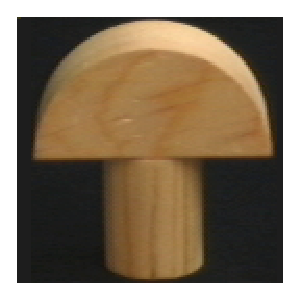
\includegraphics[width=2cm]{coil/beeld-0.eps} &
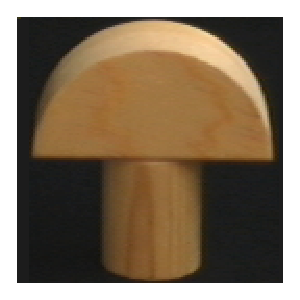
\includegraphics[width=2cm]{coil/beeld-1.eps} &
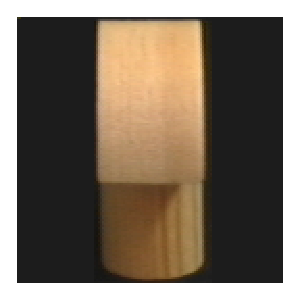
\includegraphics[width=2cm]{coil/beeld-2.eps} &
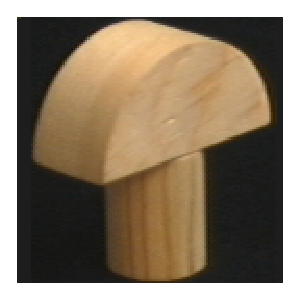
\includegraphics[width=2cm]{coil/beeld-3.eps} &
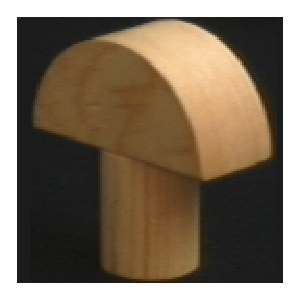
\includegraphics[width=2cm]{coil/beeld-4.eps} &
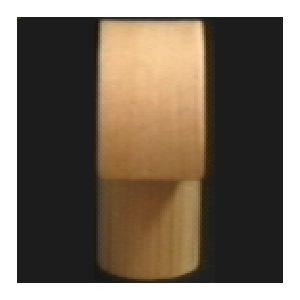
\includegraphics[width=2cm]{coil/beeld-5.eps} \\

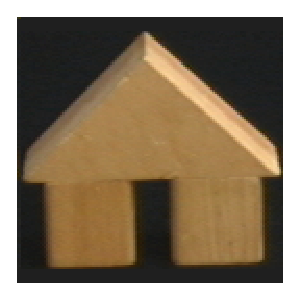
\includegraphics[width=2cm]{coil/beeld-42.eps} &
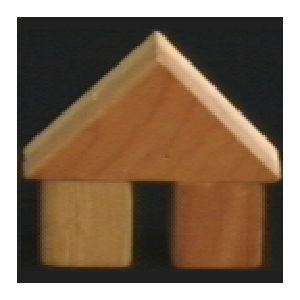
\includegraphics[width=2cm]{coil/beeld-43.eps} &
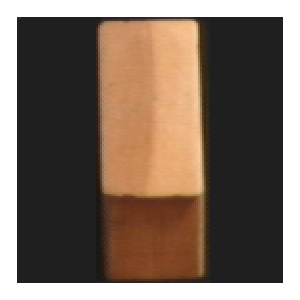
\includegraphics[width=2cm]{coil/beeld-44.eps} &
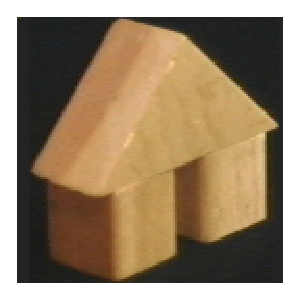
\includegraphics[width=2cm]{coil/beeld-45.eps} &
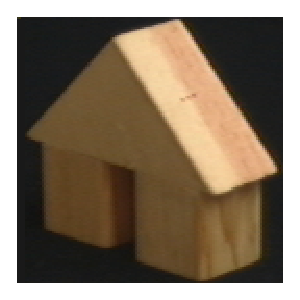
\includegraphics[width=2cm]{coil/beeld-46.eps} &
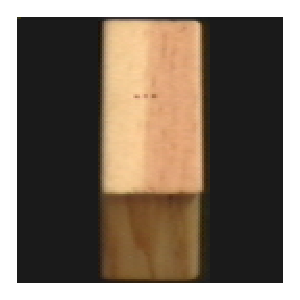
\includegraphics[width=2cm]{coil/beeld-47.eps} \\

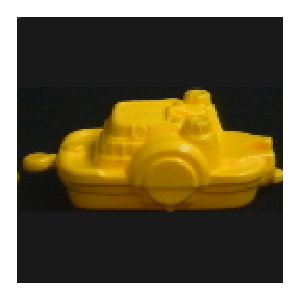
\includegraphics[width=2cm]{coil/beeld-12.eps} &
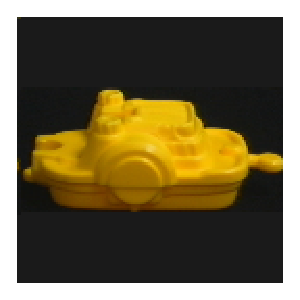
\includegraphics[width=2cm]{coil/beeld-13.eps} &
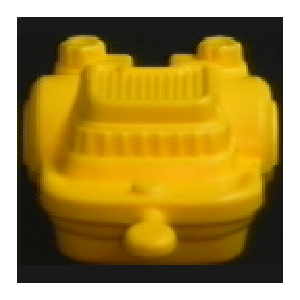
\includegraphics[width=2cm]{coil/beeld-14.eps} &
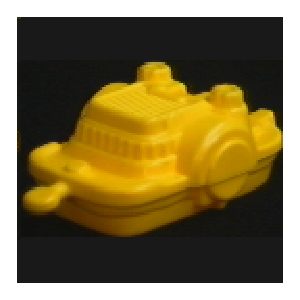
\includegraphics[width=2cm]{coil/beeld-15.eps} &
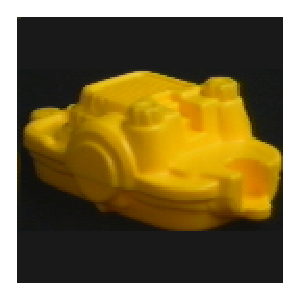
\includegraphics[width=2cm]{coil/beeld-16.eps} &
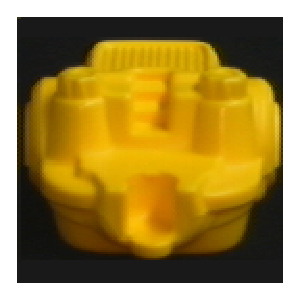
\includegraphics[width=2cm]{coil/beeld-17.eps} \\


\includegraphics[width=2cm]{coil/beeld-18.eps} &
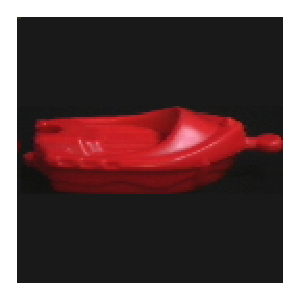
\includegraphics[width=2cm]{coil/beeld-19.eps} &
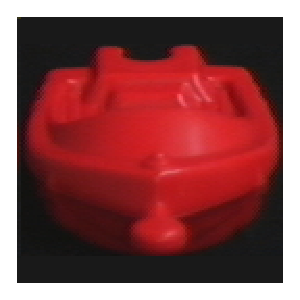
\includegraphics[width=2cm]{coil/beeld-20.eps} &
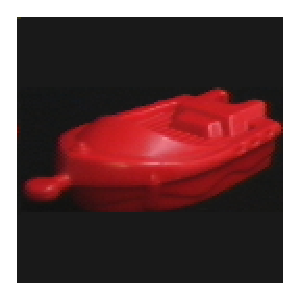
\includegraphics[width=2cm]{coil/beeld-21.eps} &
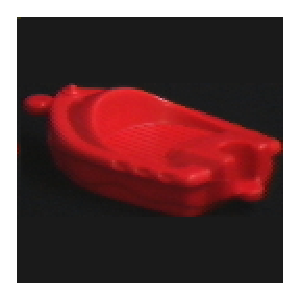
\includegraphics[width=2cm]{coil/beeld-22.eps} &
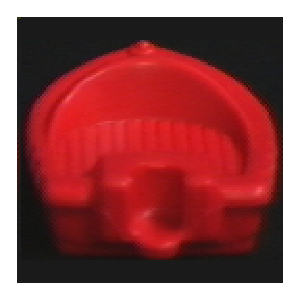
\includegraphics[width=2cm]{coil/beeld-23.eps} \\

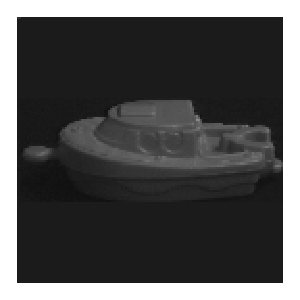
\includegraphics[width=2cm]{coil/beeld-24.eps} &
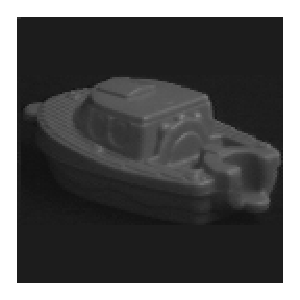
\includegraphics[width=2cm]{coil/beeld-25.eps} &
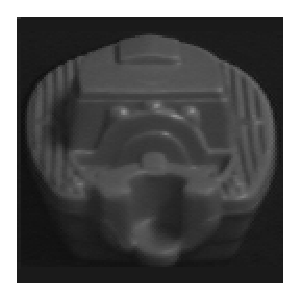
\includegraphics[width=2cm]{coil/beeld-26.eps} &
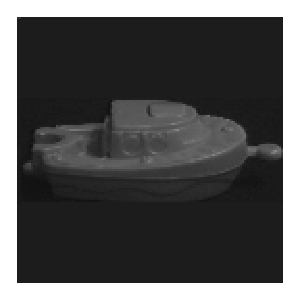
\includegraphics[width=2cm]{coil/beeld-27.eps} &
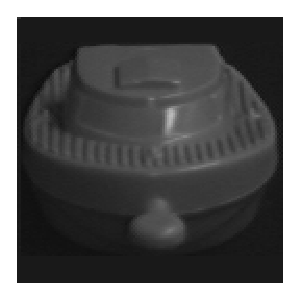
\includegraphics[width=2cm]{coil/beeld-28.eps} &
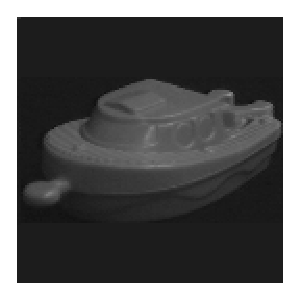
\includegraphics[width=2cm]{coil/beeld-29.eps} \\

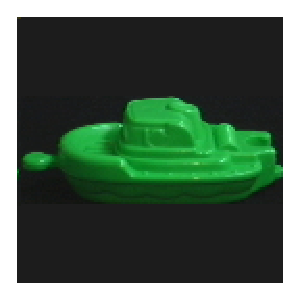
\includegraphics[width=2cm]{coil/beeld-54.eps} &
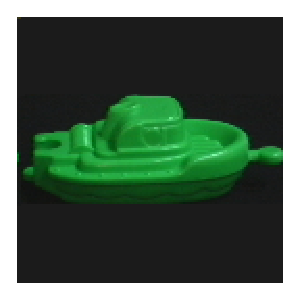
\includegraphics[width=2cm]{coil/beeld-55.eps} &
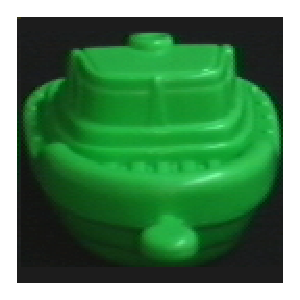
\includegraphics[width=2cm]{coil/beeld-56.eps} &
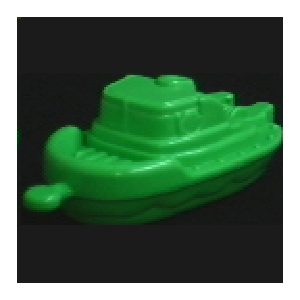
\includegraphics[width=2cm]{coil/beeld-57.eps} &
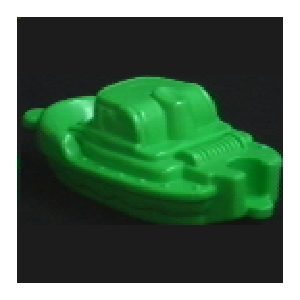
\includegraphics[width=2cm]{coil/beeld-58.eps} &
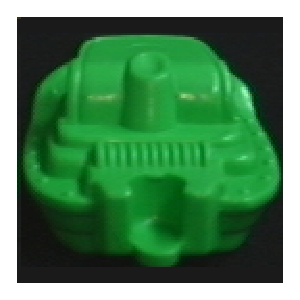
\includegraphics[width=2cm]{coil/beeld-59.eps} \\

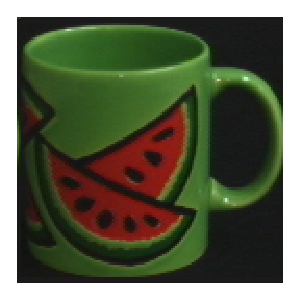
\includegraphics[width=2cm]{coil/beeld-30.eps} &
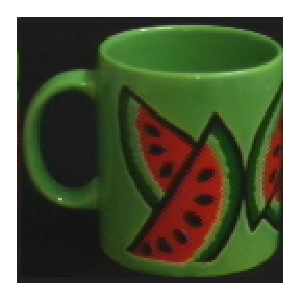
\includegraphics[width=2cm]{coil/beeld-31.eps} &
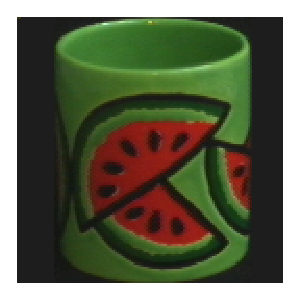
\includegraphics[width=2cm]{coil/beeld-32.eps} &
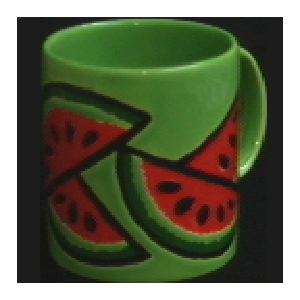
\includegraphics[width=2cm]{coil/beeld-33.eps} &
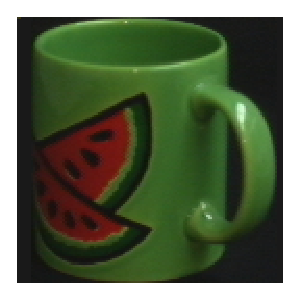
\includegraphics[width=2cm]{coil/beeld-34.eps} &
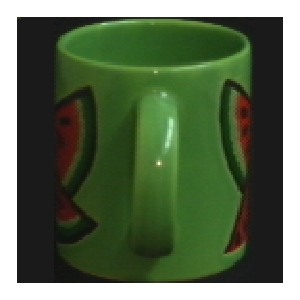
\includegraphics[width=2cm]{coil/beeld-35.eps} \\

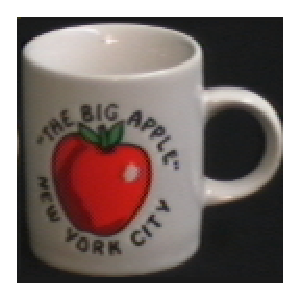
\includegraphics[width=2cm]{coil/beeld-36.eps} &
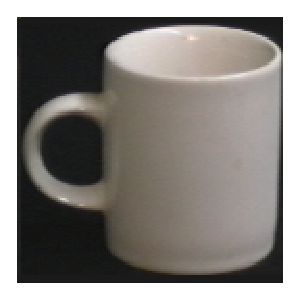
\includegraphics[width=2cm]{coil/beeld-37.eps} &
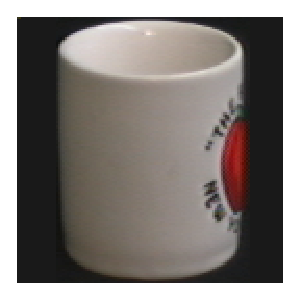
\includegraphics[width=2cm]{coil/beeld-38.eps} &
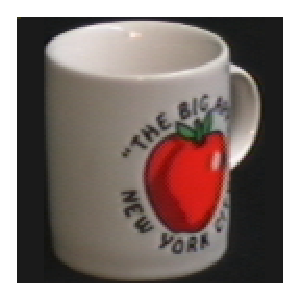
\includegraphics[width=2cm]{coil/beeld-39.eps} &
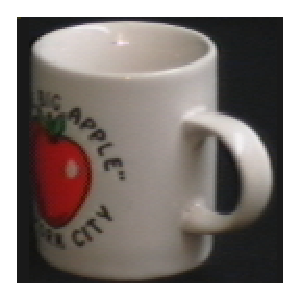
\includegraphics[width=2cm]{coil/beeld-40.eps} &
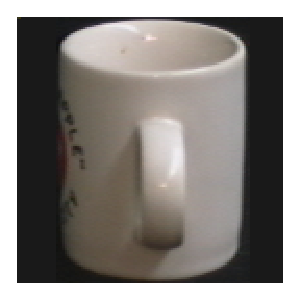
\includegraphics[width=2cm]{coil/beeld-41.eps} \\

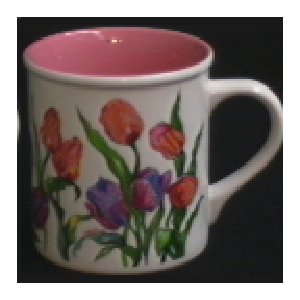
\includegraphics[width=2cm]{coil/beeld-6.eps} &
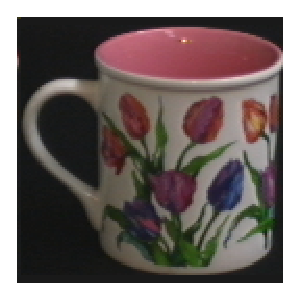
\includegraphics[width=2cm]{coil/beeld-7.eps} &
\includegraphics[width=2cm]{coil/beeld-8.eps} &
\includegraphics[width=2cm]{coil/beeld-9.eps} &
\includegraphics[width=2cm]{coil/beeld-10.eps} &
\includegraphics[width=2cm]{coil/beeld-11.eps} \\

\includegraphics[width=2cm]{coil/beeld-48.eps} &
\includegraphics[width=2cm]{coil/beeld-49.eps} &
\includegraphics[width=2cm]{coil/beeld-50.eps} &
\includegraphics[width=2cm]{coil/beeld-51.eps} &
\includegraphics[width=2cm]{coil/beeld-52.eps} &
\includegraphics[width=2cm]{coil/beeld-53.eps} \\

\includegraphics[width=2cm]{coil/beeld-60.eps} &
\includegraphics[width=2cm]{coil/beeld-61.eps} &
\includegraphics[width=2cm]{coil/beeld-62.eps} &
\includegraphics[width=2cm]{coil/beeld-63.eps} &
\includegraphics[width=2cm]{coil/beeld-64.eps} &
\includegraphics[width=2cm]{coil/beeld-65.eps} \\

\end{tabular}
\caption{\label{fig:testcollectie}De gebruikte collectie van beelden.}
\end{center}
\end{figure}

Voor het beoordelen van een rangschikking, gebruiken we de \emph{genormaliseerde gemiddelde rang} 
(GGR) \cite{muller:perf_eval}. Die performantiemaat wordt toegepast op een collectie
van $N$ beelden. Voor elk van die beelden bevat de collectie
$N_R$ zogenaamde \emph{relevante beelden}. In het geval van onze testcollectie geldt $N = 66$.
We gaan er in die collectie van uit dat foto's van eenzelfde object relevant zijn ten opzichte
van elkaar: $N_R = 6$. Beschouw nu de vector 
$(r_1,r_2,\ldots,r_{N_R}) \in \{1,2,\ldots,N\}^{N_R}$, waarbij $r_i$ het
rangnummer van het $i$-de relevante beeld voorstelt. De performantiemaat
wordt dan als volgt gedefinieerd:
\begin{definitie}
De genormaliseerde gemiddelde rang wordt gegeven door de volgende afbeelding:
\begin{displaymath}
\begin{array}{lrcl}
\textrm{GGR}: 	& \{1,2,\ldots,N\}^{N_R} & \to 	& [0,1] \\
		& (r_1,r_2,\ldots,r_{N_R}) & \mapsto &
	{\displaystyle\frac{1}{N \cdot N_R}\left[ \left(\sum_{i=1}^{N_R}r_i\right) - \frac{N_R \cdot (N_R + 1)}{2} \right]},\\[15pt]
	& & & \qquad \quad \forall (r_1, r_2, ..., r_{N_R}) \in \{1,2,\ldots,N\}^{N_R}
\end{array}
\end{displaymath}
\end{definitie}
\noindent
Deze maat nadert naar 1 naarmate de performantie slechter wordt.

Tot nu toe hebben we er nog geen rekening mee gehouden dat de performantie van
een similariteitsmaat afhankelijk kan zijn van het gekozen voorbeeld. Dat probleem lossen we
op door de GGR te berekenen voor meerdere voorbeelden en het gemiddelde van de bekomen waarden
te beschouwen. We kiezen daarbij de beelden uit de linker kolom van 
figuur~\ref{fig:testcollectie} als voorbeeld. De waarde die we zo bekomen noemen we de
\emph{globale genormaliseerde gemiddelde rang} (GGGR). Het is die waarde die we zullen gebruiken
om de performantie van een similariteitsmaat te evalueren. We zullen dus met andere woorden op
zoek gaan naar similariteitsmaten waarvan de GGGR zo klein mogelijk is.

\subsection{Rekentijd}

Voor elke similariteitsmaat die we construeren meten we ook hoe lang het duurt om
de rangschikkingen, die nodig zijn om de GGGR te bepalen, te berekenen. Aan die 
rekentijd hechten we echter niet zoveel belang als aan de GGGR, vermits het in onze
praktische implementatie niet absoluut noodzakelijk is dat de similariteitsmaten zo weinig
mogelijk rekentijd vereisen. De collecties van beelden waarop ze daarbij toegepast worden,
zijn immers beperkt in grootte. Bovendien worden de berekeningen aan de kant van de client
uitgevoerd, waardoor er geen gevaar is voor overbelasting van de server.

Indien we de similariteitsmaten zouden construeren voor een zuiver CBIR-systeem, zoals weergegeven
in figuur~\ref{fig:cbir}, dan zou de rekentijd wel zeer belangrijk zijn. Hoewel het aantal
beelden beperkt wordt door het gebruik van multidimensionale indexering, zal een dergelijk
systeem de similariteitsmaten immers toch nog moeten toepassen op een groot aantal
beelden. Anderzijds laat een zuiver CBIR-systeem wel toe om berekeningen op voorhand te doen
en de resultaten ervan samen met de beelden op te slaan in de databank. Bij het similariteitsgebaseerd
rangschikken van de zoekresultaten is dat niet mogelijk, omdat de databank daarbij niet rechtstreeks
toegankelijk is.

Als we het bepalen van de similariteiten vergelijken met het studeren voor een examen, dan 
heeft de student in het geval van echte CBIR op voorhand meer dan voldoende tijd om de leerstof
te verwerken. Vlak voor het examen is er echter maar net genoeg tijd om alles nog eens 
te herhalen. Bij het similariteitsgebaseerd rangschikken van de zoekresultaten kan er niet vooraf 
gestudeerd worden, maar juist voor het examen heeft de student wel nog enkele dagen ter beschikking 
om alles in te studeren.


\section{Beperken van de rekentijd}
\label{sectie:beperken_rekentijd}

Hoewel de rekentijd voor onze praktische toepassing niet van cruciaal belang is, kan het beperken 
ervan uiteraard geen kwaad. Door toch voldoende aandacht te schenken aan de rekentijd kunnen
we er zelfs voor zorgen dat similariteitsmaten waarvoor we zonder extra inspanning veel te lang zouden 
moeten rekenen, toch nog bruikbaar zijn.

Stel dat $A$ en $B$ twee vaagverzamelingen zijn in een zelfde universum $X$. Het kan dan voorkomen dat 
$X'= supp\ A \cup supp\ B$ veel minder elementen bevat dan $X$. In dat geval kunnen we de rekentijd sterk
reduceren door het bereik van de sommaties in de vaagsimilariteitsmaten te beperken tot $X'$. Doordat
$A(x)=B(x)=0$ voor alle $x \in X \setminus X'$ geldt er dan immers zowel
\begin{align*}
\displaystyle \sum_{x \in X} | A(x) - B(x) | 
&= \displaystyle \sum_{x \in X \setminus X'} | A(x) - B(x) | + \displaystyle \sum_{x \in X'} | A(x) - B(x) | \\
&= \displaystyle \sum_{x \in X \setminus X'} | 0 - 0 | + \displaystyle \sum_{x \in X'} | A(x) - B(x) | \\
&= \displaystyle \sum_{x \in X'} | A(x) - B(x) |
\end{align*}
als $|A| = \sum_{x \in X} A(x) = \sum_{x \in X \setminus X'} 0 + \sum_{x \in X'} A(x) 
= \sum_{x \in X'} A(x)$.
% \begin{displaymath}
% |A| = \sum_{x \in X} A(x) = \sum_{x \in X \setminus X'} A(x) + \sum_{x \in X'} A(x) 
% = \sum_{x \in X \setminus X'} 0 + \sum_{x \in X'} A(x) = \sum_{x \in X'} A(x)
% \end{displaymath}
Wanneer we $||A|| = \sum_{x \in X'} A(x)$ defini\"eren, dan geldt dus $|A| = ||A||$ en ook:
\begin{align*}
| A \cap B | 
&= \displaystyle \sum_{x \in X} T_M(A(x),B(x)) & & \\
&= \displaystyle \sum_{x \in X'} T_M(A(x),B(x)) & & (T_M(0,0)=0) \\
&= ||A \cap B|| & & \displaybreak[0] \\ %[5pt]
| A \cup B | 
&= \displaystyle \sum_{x \in X} S_M(A(x),B(x)) & & \\
&= \displaystyle \sum_{x \in X'} S_M(A(x),B(x)) & & (S_M(0,0)=0) \\
&=  ||A \cup B|| & & \displaybreak[0] \\ %[5pt]
| A \setminus B | = | A \cap B^c | 
&= \displaystyle \sum_{x \in X} T_M(A(x),1-B(x)) & & \\
&= \displaystyle \sum_{x \in X'} T_M(A(x),1-B(x)) & & (T_M(0,1-0)=T_M(0,1)=0) \\
&= || A \cap B^c || = ||A \setminus B|| & & %\\[5pt]
\end{align*}
Doordat $T_M(0,1)=0$ en $S_M(0,0)=0$ geldt eveneens
% \begin{align*}
% | A \triangle B | 
% &= | (A \setminus B) \cup (B \setminus A) | & & \\
% &= || (A \setminus B) \cup (B \setminus A) || & & (T_M(0,1)=0 \textrm{ en } S_M(0,0)=0) \\
% &= || A \triangle B || & & \\
% \end{align*}
\begin{displaymath}
| A \triangle B | = | (A \setminus B) \cup (B \setminus A) | = || (A \setminus B) \cup (B \setminus A) || = || A \triangle B ||
\end{displaymath}
% \end{align*}
en uit $T_M(0,1)=0$ volgt dat 
% \begin{align*}
% |(A \cap B) \cap (A^c \cap B^c)| &= ||(A \cap B) \cap (A^c \cap B^c)|| & & (T_M(0,1)=0)\\ %[5pt]
% |(A \cup B) \cap (A^c \cup B^c)| &= ||(A \cup B) \cap (A^c \cup B^c)|| & & (T_M(0,1)=0)
% \end{align*}
$|(A \cap B) \cap (A^c \cap B^c)| &= ||(A \cap B) \cap (A^c \cap B^c)||$ en
$|(A \cup B) \cap (A^c \cup B^c)| &= ||(A \cup B) \cap (A^c \cup B^c)||$.
Met behulp van de eigenschap
\begin{displaymath}
|A^c| = \sum_{x \in X} (1 - A(x)) = \sum_{x \in X} 1 - \sum_{x \in X} A(x) = |X| - |A|
\end{displaymath}
vinden we bovendien:
\begin{displaymath}
\begin{array}{l@{\ =\ }l@{\ =\ }l@{\ =\ }l}
|A^c \cap B^c| & |(A \cup B)^c| & |X| - |A \cup B| & |X| - ||A \cup B|| \\[4pt]
|A^c \cup B^c| & |(A \cap B)^c| & |X| - |A \cap B| & |X| - ||A \cap B||
\end{array}
\end{displaymath}
\begin{displaymath}
\begin{array}{l@{\ =\ }l@{\ =\ }l}
| (A \setminus B)^c | & |X| - |A \setminus B| & |X| - ||A \setminus B|| \\[4pt]
| (A \triangle B)^c | & |X| - |A \triangle B| & |X| - ||A \triangle B||
\end{array}
\end{displaymath}
\begin{displaymath}
\begin{array}{l@{\ =\ }l@{\ =\ }l}
|(A^c \cap B^c) \cup (A \cap B)| & |((A \cup B) \cap (A^c \cup B^c))^c| & |X| - ||(A \cup B) \cap (A^c \cup B^c)|| \\[4pt]
|(A^c \cup B^c) \cup (A \cup B)| & |((A \cap B) \cap (A^c \cap B^c))^c| & |X| - ||(A \cap B) \cap (A^c \cap B^c)||
\end{array}
\end{displaymath}
We kunnen tabel~\ref{tab:similatiteitsmaten} bijgevolg herschrijven tot tabel~\ref{tab:beperkte_similatiteitsmaten}.
\begin{table}[!t]
\begin{center}
\begin{tabular}{|l|}
\hline
\\[1pt]
$
\begin{array}{r@{\ }c@{\ }l}
\displaystyle M_{1a}(A,B) & = & \displaystyle 1-\frac{1}{|X|}\sum_{x \in X'} | A(x) - B(x) | \\
\displaystyle M_{1b}(A,B) & = & \displaystyle 1-\left(\frac{1}{|X|}\sum_{x \in X'} | A(x) - B(x) |^2\right)^\frac{1}{2} \\
\displaystyle M_{1c}(A,B) & = & \displaystyle 1-\left(\frac{1}{|X|}\sum_{x \in X'} | A(x) - B(x) |^4\right)^\frac{1}{4} \\
\end{array}
\begin{array}{r@{\ }c@{\ }l}
\displaystyle M_2(A,B) & = & \displaystyle 1 - \max_{x \in X'} | A(x) - B(x) | \\[10pt]
\displaystyle M_3(A,B) & = & \displaystyle 1 - \frac{\displaystyle \sum_{x \in X'} | A(x) - B(x) |}{\displaystyle ||A|| + ||B||} \\
\end{array}
$
\\
\\[1pt]
\hline
\\[1pt]
$
\begin{array}{r@{\ }c@{\ }l}
\displaystyle M_5(A,B) & = & \displaystyle \frac{\min \{||A||,||B||\}}{\max \{||A||,||B||\}} \\[10pt]
\displaystyle M_{5c}(A,B) & = & \displaystyle \frac{|X|-\max \{||A||,||B||\}}{|X|-\min \{||A||,||B||\}} \\[10pt]
\displaystyle M_6(A,B) & = & \displaystyle \frac{||A \cap B||}{||A \cup B||} \\[10pt]
\displaystyle M_{6c}(A,B) & = & \displaystyle \frac{|X|-||A \cup B||}{|X|-||A \cap B||} \\[10pt]
\displaystyle M_7(A,B) & = & \displaystyle \frac{||A \cap B||}{\max \{||A||,||B||\}} \\[10pt]
\displaystyle M_{7c}(A,B) & = & \displaystyle \frac{|X|-||A \cup B||}{|X|-\min \{||A||,||B||\}} \\[10pt]
\displaystyle M_8(A,B) & = & \displaystyle \frac{||A \cap B||}{\min \{||A||,||B||\}} \\[10pt]
\displaystyle M_{8c}(A,B) & = & \displaystyle \frac{|X|-||A \cup B||}{|X|-\max \{||A||,||B||\}} \\[10pt]
\end{array}
\begin{array}{@{\qquad}r@{\ }c@{\ }l}
\displaystyle M_9(A,B) & = & \displaystyle \frac{\min \{||A||,||B||\}}{||A \cup B||} \\[10pt]
\displaystyle M_{9c}(A,B) & = & \displaystyle \frac{|X| - \max \{||A||,||B||\}}{|X| - ||A \cap B||} \\[10pt]
\displaystyle M_{10}(A,B) & = & \displaystyle \frac{\max \{||A||,||B||\}}{||A \cup B||} \\[10pt]
\displaystyle M_{10c}(A,B) & = & \displaystyle \frac{|X| - \min \{||A||,||B||\}}{|X| - ||A \cap B||} \\[10pt]
\displaystyle M_{11}(A,B) & = & \displaystyle \frac{\min \{||A \setminus B||,||B \setminus A||\}}{\max \{||A \setminus B||,||B \setminus A||\}} \\[10pt]
\displaystyle M_{11c}(A,B) & = & \displaystyle \frac{|X| - \max \{||A \setminus B||,||B \setminus A||\}}{|X| - \min \{||A \setminus B||,||B \setminus A||\}} \\[10pt]
\displaystyle M_{12}(A,B) & = & \displaystyle \frac{|X| - ||A \triangle B||}{|X|-\min \{||A \setminus B||,||B \setminus A||\}} \\[10pt]
\displaystyle M_{13}(A,B) & = & \displaystyle \frac{|X|-||A \triangle B||}{|X|-\max \{||A \setminus B||,||B \setminus A||\}}
\end{array}
$
\\
\\[1pt]
\hline
\\[1pt]
$
\begin{array}{r@{\ }c@{\ }l}
\displaystyle M_{I_3}(A,B) & = & \displaystyle \frac{||(A \cap B) \cap (A^c \cap B^c)||}{||(A \cup B) \cap (A^c \cup B^c)||}
\end{array}
\begin{array}{@{\qquad}r@{\ }c@{\ }l}
\displaystyle M_{I_{3c}}(A,B) & = & \displaystyle \frac{|X| - ||(A \cup B) \cap (A^c \cup B^c)||}{|X|-||(A \cap B) \cap (A^c \cap B^c)||}
\end{array}
$
\\
\\[1pt]
\hline
\end{tabular}
\caption{\label{tab:beperkte_similatiteitsmaten}De vaagsimilariteitsmaten geschreven met sommaties waarvan het bereik beperkt is.}
\end{center}
\end{table}
% beter geen nieuwe paragraaf volgens Valerie
Beschouw bijvoorbeeld $M_{5}$:
\begin{displaymath}
M_{5} = \frac{\min\{|A|,|B|\}}{\max\{|A|,|B|\}} = \frac{\min\{||A||,||B||\}}{\max\{||A||,||B||\}}
\end{displaymath}
Bij de oude formule zijn er eerst $2 \cdot (|X|-1)$ optellingen nodig
om $|A|$ en $|B|$ te berekenen. Daarna moeten de zo bekomen getallen met elkaar vergeleken worden
om $\min\{|A|,|B|\}$ en $\max\{|A|,|B|\}$ te bepalen en moet er tenslotte ook nog \'e\'en deling
uitgevoerd worden. De herschreven vorm vereist $ 2 \cdot (|X'|-1)$ optellingen, \'e\'en vergelijking
en \'e\'en deling. Vermits $|X'| \ll |X|$ impliceert 
dat $2 \cdot (|X'|-1) + 2 \ll 2 \cdot (|X|-1) + 2$, zal de nieuwe formule inderdaad een stuk sneller kunnen 
berekend worden dan de oude als $X'$ veel minder elementen bevat dan $X$. Bovendien zijn de rekentijden
gelijk als $X'=X$. De nieuwe vorm is dus steeds minstens even snel als de oude.

Bij de vaagsimilariteitsmaten die gebruik maken van het complement, boeken we nog meer winst.
We bekijken $M_{5c}$ als voorbeeld. De oorspronkelijke vorm wordt als volgt herschreven:
\begin{align*}
\displaystyle M_{5c}(A,B) = \displaystyle \frac{\min \{|A^c|,|B^c|\}}{\max \{|A^c|,|B^c|\}} 
& = \displaystyle \frac{\min \{|X|-||A||,|X|-||B||\}}{\max \{|X|-||A||,|X|-||B||\}} \\
& = \displaystyle \frac{|X| + \min \{-||A||,-||B||\}}{|X| + \max \{-||A||,-||B||\}} \\
& = \displaystyle \frac{|X| - \max \{||A||,||B||\}}{|X| - \min \{||A||,||B||\}}
\end{align*}
Voor de oude formule zijn er $2\cdot |X|$ aftrekkingen nodig om $A^c$ en $B^c$ te bepalen,
bovenop de $2 \cdot (|X|-1) + 2$ bewerkingen die nodig zijn voor het berekenen van 
%$\min\{|A|,|B|\} / \max\{|A|,|B|\}$. 
de originele vorm van $M_5$. De nieuwe formule daarentegen vereist slechts twee bewerkingen
meer dan de herschreven vorm van $M_5$. Zelfs voor $|X'| = |X|$ zal 
$2 \cdot |X| + 2 \cdot (|X|-1) + 2 = 4 \cdot |X|$ doorgaans een stuk groter zijn dan
$2 \cdot (|X'|-1) + 4 = 2 \cdot |X'| + 2$. Als $|X'| \ll |X|$ dan wordt het verschil in rekentijd
uiteraard nog significanter.

Merk op dat we in de bovenstaande redeneringen enkel gesteund hebben op $T_M(0,0)=T_M(0,1)=0$ en 
$S_M(0,0)=0$. 
De bekomen eigenschappen blijven dus gelden indien we $T_M$ en $S_M$ vervangen door respectievelijk 
een willekeurige conjunctor $\mathcal{C}$ en een willekeurige disjunctor $\mathcal{D}$, waarvoor per 
definitie geldt: $\mathcal{C}(0,0)=\mathcal{C}(0,1)=\mathcal{C}(1,0)=0$ en $\mathcal{D}(0,0)=0$. 